\documentclass{jfpda}

%\newcommand{\verbfichex}{jfpda.\xspace}
%\newcommand{\verbfichclass}{jfpda.cls\xspace}
%\newcommand{\verbfichbst}{jfpda.bst\xspace}

% Packages
\usepackage[pdftex]{pstricks}
\usepackage{verbatim}
\usepackage{graphicx}
\usepackage[algo2e,vlined,ruled]{algorithm2e}
\usepackage{amssymb}
\usepackage{amsmath}
\usepackage{epstopdf}
%\usepackage{amsthm}
%\usepackage[T1]{fontenc}
\usepackage{natbib}

\shorttitle{Q-Learning for Autonomous Soaring}

\shortouvrage{JFPDA 2017}

\title{Empirical evaluation of a Q-Learning Algorithm for Model-free Autonomous Soaring}

\author{Erwan Lecarpentier\inst{1,}, Sebastian Rapp\inst{2,}, Marc Melo, Emmanuel Rachelson\inst{3,}}

\institute{
	ONERA -- DTIS (D\'{e}partement du Traitement de l'Information et Syst\`{e}mes) \\
	2 avenue Edouard Belin, 31000 Toulouse, France \\
	\texttt{erwan.lecarpentier@isae.fr}
	\and
	TU Delft -- Department of Aerodynamics, Wind Energy \& Propulsion \\
	Building 62, room B62-5.07, Kluyverweg 1, 2629 HS Delft, Netherlands \\
	\texttt{s.rapp@tudelft.nl}
	\and
	ISAE Supaero -- DISC (D\'{e}partement d'Ing\'{e}nierie des Syst\`{e}mes Complexes)\\
	10 avenue Edouard Belin, 31055 Toulouse, France\\
	\texttt{emmanuel.rachelson@isae.fr}
}

\begin{document}

\maketitle

\begin{abstract}
	Autonomous unpowered flight is a challenge for control and guidance systems: all the energy the aircraft might use during flight has to be harvested directly from the atmosphere.
	We investigate the design of an algorithm that optimizes the closed-loop control of a glider's bank and sideslip angles, while flying in the lower convective layer of the atmosphere in order to increase its mission endurance.
	Using a Reinforcement Learning approach, we demonstrate the possibility for real-time adaptation of the glider's behavior to the time-varying and noisy conditions associated with thermal soaring flight.
	Our approach is online, data-based and model-free, hence avoids the pitfalls of aerological and aircraft modeling and allow us to deal with uncertainties and non-stationarity.
	Additionally, we put a particular emphasis on keeping low computational requirements in order to make on-board execution feasible.
	This article presents the stochastic, time-dependent aerological model used for simulation, together with a standard aircraft model. Then we introduce an adaptation of a $Q$-learning algorithm and demonstrate its ability to control the aircraft and improve its endurance by exploiting updrafts in non-stationary scenarios.
	
	\motscles{Reinf\label{key}orcement learning control, Adaptive control applications, Adaptation and learning in physical agents, UAVs.}
\end{abstract}

\section{INTRODUCTION}

The number of both civil and military applications of small unmanned aerial vehicles (UAVs) has augmented during the past few years. However, as the complexity of their tasks is increasing, extending the range and flight duration of UAVs becomes a key issue. Since the size, and thus the energy storage capacity, is a crucial limiting factor, other means to increase the flight duration have to be examined. A promising alternative is the use of atmospheric energy in the form of gusts and updrafts. This could significantly augment the mission duration while simultaneously save fuel or electrical energy. For this reason, there is a great interest in the development of algorithms that optimize the trajectories of soaring UAVs by harvesting the energy of the atmosphere. Since the atmospheric conditions are changing over time, it is crucial to develop an algorithm able to find an optimal compromise between exploring and exploiting convective thermal regions, while constantly adapting itself to the changing environment.
%the large amount of uncertainties in the aircraft dynamics as well as in the environmental model.
%adapting the command to the aircraft dynamics and the environment supposedly unknown.

In this work we adapt a $Q$-learning \cite{watkins92qlearning} algorithm for this task. Our method is model-free, therefore suitable for a large range of environments and aircrafts. Additionally, it does not need pre-optimization or pre-training, works in real-time, and can be applied online. Although the gap towards a fully autonomous physical demonstrator has not been bridged yet, our main contribution in this work is the \emph{proof of concept} that a model-free reinforcement learning approach can efficiently enhance a glider's endurance.
We start by reviewing the state of the art in UAV static soaring and thermal modeling in Section \ref{sec:relwork} and position our contributions within previous related work. Then, in Section \ref{sec:atmos}, we present the specific atmospheric model we used and its improvements over previous contributions, along with the thermals scenario used in later experiments. Section \ref{sec:aircraft} details the aircraft dynamics model. We introduce our implementation of the $Q$-learning algorithm in Section \ref{sec:control} and discuss its strengths, weaknesses and specific features. Simulation results are presented in Section \ref{sec:results}. We finally discuss the limitations of our approach and conclude in Section \ref{sec:conclu}.

\section{RELATED WORK}
\label{sec:relwork}

During the last decade, several possibilities to efficiently utilize atmospheric energy for soaring aircrafts have been proposed. For a general introduction to static and dynamic soaring, refer to \cite{chen1981} for instance. For a more specific review on thermal centering and soaring in practice, see \cite{reichmann}.

Most approaches to thermal soaring rely on the identification of some model of the wind field surrounding the aircraft. This estimated wind field is then used to track an optimized trajectory inside the thermal or between thermals, using various methods for identification and path planning \cite{allen05,allen07,lawrance11,lawrance_phd,bencatel13,chen11,chakrabarty}. Such approaches demonstrated important energy savings (up to 90\% in simulation \cite{chakrabarty}) compared to conventional flight. A alternative robust control algorithm \cite{kahveci}, based again on a pre-identification of a thermal model showed good results also.

%% Most approaches to thermal soaring rely on the identification of some model of the wind field surrounding the aircraft. \cite{allen05} detects thermals by monitoring accelerations and pressure, and identifying a predefined thermal model. Predefined trajectory patterns are then applied. \cite{allen07} estimate thermal parameters and relative position to the glider which are in turn used to track an optimal trajectory inside a thermal. In their work, a mode logic was developed to switch between soaring and searching flight. \cite{lawrance11} use Gaussian Processes regression to calculate {\color{red}(estimate ?)} the mean and variance of a wind field. They exploit this knowledge to rank trajectories with respect to mission goals. Based on similar ideas, in \cite{lawrance_phd}, a path planning architecture for autonomous soaring flight in unknown wind fields has been developed. Similar ideas can be found in \cite{bencatel13} or \cite{chen11}, whose approach showed energy savings of up to 90\% in simulation compared to conventional flights. In the path planning literature, \cite{chakrabarty} adapt an $A^*$ algorithm to the search for an optimal trajectory in a known wind field. Finally, to cope with model uncertainties, \cite{kahveci} introduce a robust adaptive control algorithm taking into account the changing flight and environmental conditions.
%% % To address actuator saturation, an LMI-based anti-windup compensator is included, which, combined with the adaptive LQ controller, allows optimal autonomous soaring performances.
%% {\color{red}Here} again, the thermal strength and position are supposed to be known, using sensor measurements and ground base data. Overall, one major disadvantage of such model-based approaches is the dependence on a thermal identification algorithm, which may not be robust enough against model inaccuracy. 

%Authors such as \cite{beeler}, \cite{bonnin13} or \cite{patel} focus on the exploitation of gusts or wind gradients. The two former generate open-loop trajectories which require the knowledge of an exact model of the system to control. The later provides a methodology to design a control law that yields good average efficiency over a certain range of gusts, but is non-adaptive. Results showed that sometimes the active control law resulted in a higher energy loss than a flight with a conventional flight controller, due to the stochastic nature of the turbulent gusts and the model-based control algorithm.

In this paper, we reconsider the possibility to use a \emph{Reinforcement Learning} (RL, \cite{sutton_book}) approach to optimize the trajectory. Using RL to exploit thermals has already been examined in \cite{wharington_phd}. In this work, a neural-based thermal center locator for the optimal autonomous exploitation of the thermals is developed. After each completed circle, the algorithm memorizes the heading where the lift was the strongest and moves the circling trajectory towards the lift. However, this thermal locator is too time consuming for real-time on-board applications.

We introduce a \emph{Q-learning} algorithm using a \emph{linear function approximation}, which is simple to implement, demands less computational resources and does not rely on the identification of a thermal model.
%It appears therefore more suited for a real-time application.
We empirically evaluate this online learning algorithm (Section \ref{sec:control}) by interfacing it with a simulation model that couples the aircraft dynamics (Section \ref{sec:aircraft}) with an improved local aerological model (Section \ref{sec:atmos}).
%This aerological model is based on the model described in \cite{allen_thermal} and further refined.
%We improved it by adding a time-dependent shape change as well as a drift velocity, which provides a more realistic simulation. 
We use the model to test our algorithm in several scenarios and show that it yields a significant endurance improvement. Our algorithm's main feature lies in its complete independence of the characteristics of the aerological environment, which makes it robust against model inaccuracy and estimation noise. Moreover, not explicitly estimating the thermal center position and updraft magnitude saves valuable computational time.

\section{ATMOSPHERIC MODEL}
\label{sec:atmos}

Our updraft model expands on \cite{allen_thermal}. Their model possesses three desirable features: dependence of the updraft distribution in the vertical direction, explicit modeling of downdrafts at the thermal's border and at every altitude, and finally the use of an environmental sink rate to ensure conservation of mass. Although a complete literature review on modeling the convective boundary layer is beyond the scope of this paper, it should be noted that \cite{allen_thermal} is the first reference that includes these three modeling aspects.

%\begin{figure}%[!ht]
%\begin{center}
% 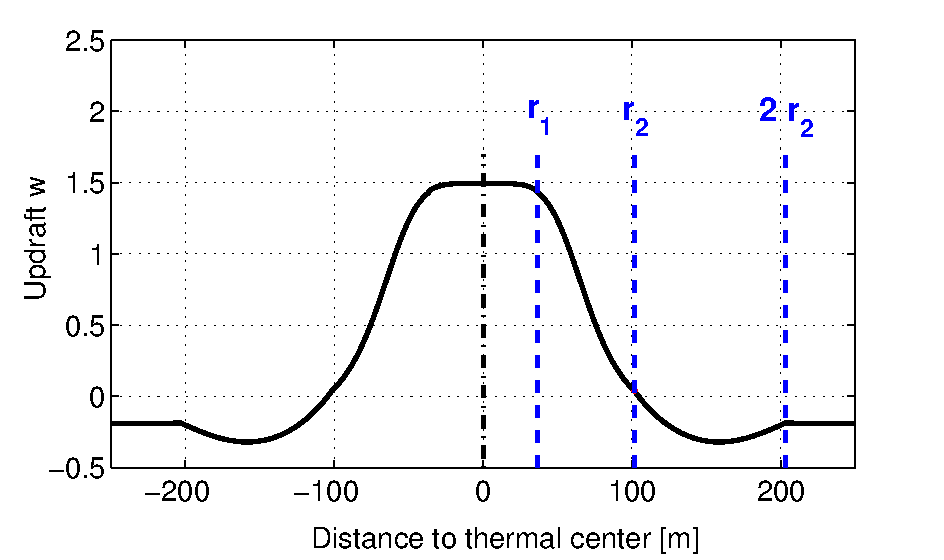
\includegraphics[width=9cm]{img/AllenThermal_radius.pdf}
% \caption{Updraft distribution example at 750m}
% \label{fig:updraft900}
%\end{center}
%\end{figure}

\begin{figure}%[!ht]
\begin{center}
 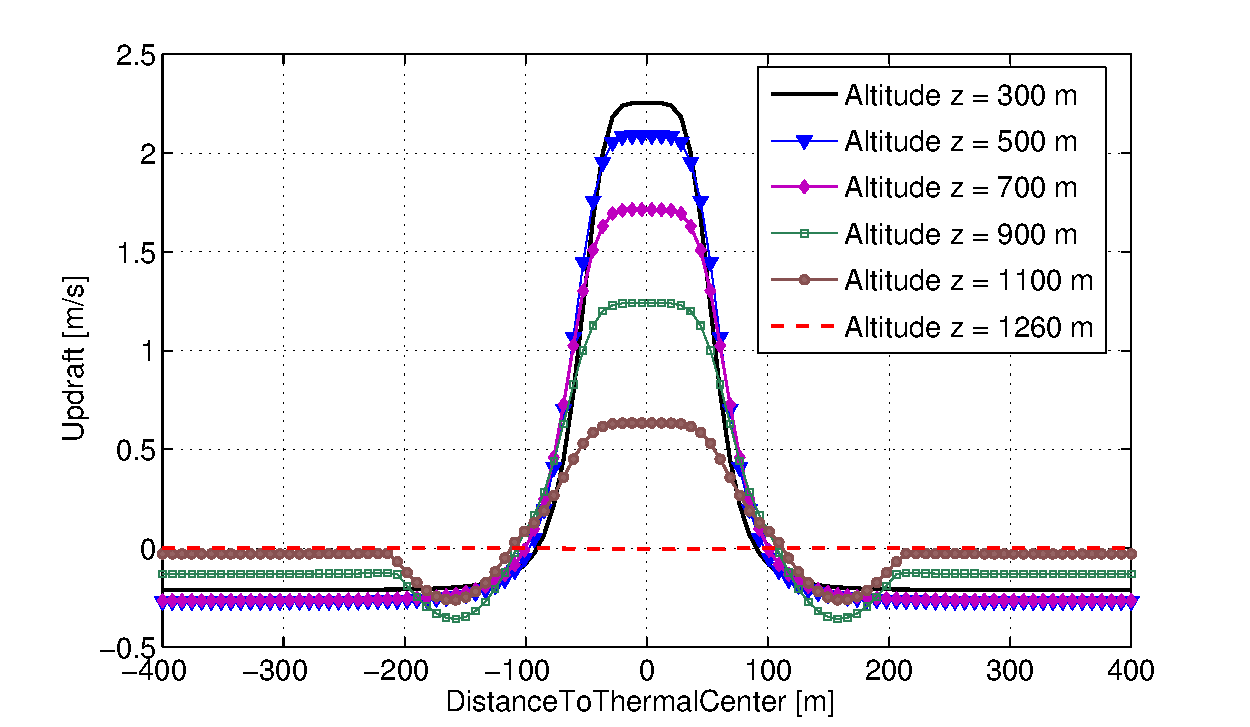
\includegraphics[width=9cm]{img/total_updraft.pdf}
\end{center}
 \caption{Updraft distribution with altitude}
 \label{fig:updraft_distribution}
\end{figure}

%\begin{figure}
%\centering 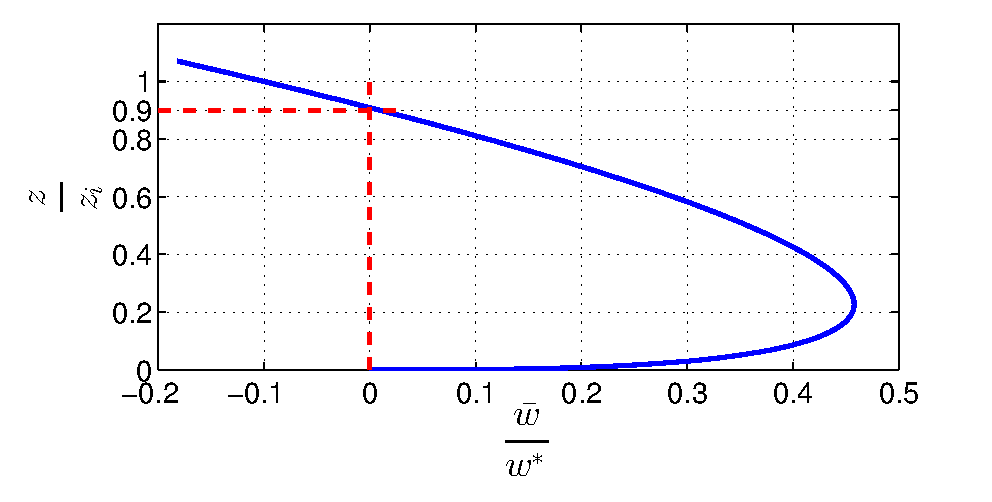
\includegraphics[width=9cm]{img/zzi_wbar.pdf}
%\caption{Updraft average velocity ratio vertical evolution}
%\label{fig:wbar}
%\end{figure}

We describe a thermal updraft as a symmetrical, bell-shaped distribution as illustrated in Figure \ref{fig:updraft_distribution}. This distribution is characterized by two radii $r_1$ and $r_2$. At a given altitude $z$, if $r$ denotes the distance to the thermal center, for $r<r_1$ the updraft has a quasi-constant value of $w_{peak}$, then for $r_1<r<r_2$ this value drops smoothly to zero, and between $r_2$ and $2r_2$ appears a downdraft. The thermal has no influence further than $2r_2$.

The maximum updraft velocity $w_{peak}$ evolves altitude-wise proportionally to $w^* \left( \frac{z}{z_i} \right)^{\frac{1}{3}} \left(1 - 1.1 \ \frac{z}{z_i}\right)$, where $w^*$ is an average updraft velocity and $z_i$ is a scaling factor indicating the convective boundary layer thickness.
%This evolution is shown in figure \ref{fig:wbar}. 
Above $0.9z_i$ all velocities are assumed to be zero.

Finally, based on the conservation of mass principle, an altitude-dependent global environmental sink rate is calculated and applied everywhere outside the thermals. For specific equations, we refer the reader to \cite{allen_thermal}.

We introduce three additional features that bring our simulation model closer to a real-life description, namely thermal drift, life-cycle and noise.
First, in order to account for local winds, we let the thermals drift in the horizontal plane with a velocity $(\bar{v}_x, \bar{v}_z)$. Usually, the root point of a thermal is a fixed location and the thermal leans with the wind, so introducing a thermal drift is a poor description of this phenomenon. Nevertheless, for our simulations, it approximates the practical phenomenon of drift given that the aircraft model is reduced to a single point-mass.
Thermals also have a finite life. We decompose a thermal's life in a latency phase of duration $t_{\textit{off}}$ and a growth, maturity and fade-off phase of duration $t_{\textit{life}}$. After $t_{\textit{off}} \, + \, t_{\textit{life}}$ the thermal dies. The life-cycle of a thermal is described by the updraft coefficient $c_\xi(t)$ shown in Figure \ref{fig:life_cycle}, using a shape parameter $\xi$. This $c_\xi(t)$ coefficient is used as a multiplier on the total updraft.
Finally, it is well-known among cross-country pilots that thermals are rarely round and present a great variety of shapes and much noise. In order to account for this fact and to model real-life uncertainties we added a Gaussian distributed noise $n$ to the wind velocity.

\begin{figure}%[!ht]
\begin{center}
 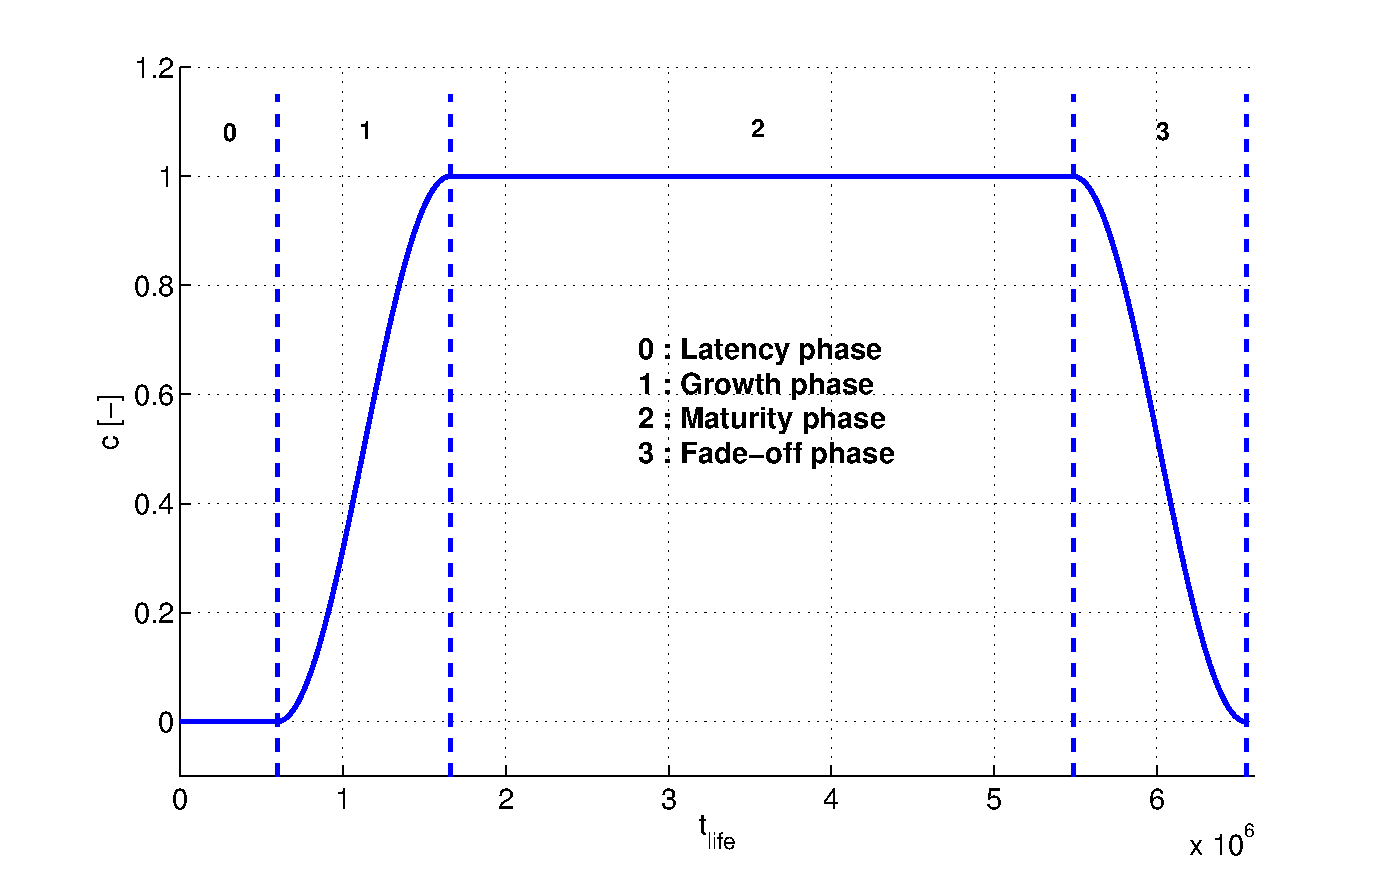
\includegraphics[width=9cm]{img/lifeCycle.pdf}
\end{center}
\caption{Evolution of the updraft coefficient $c_\xi(t)$}
\label{fig:life_cycle}
\end{figure}

We maintain a constant number $N$ of thermals in the flight area, although some might be in their latency phase. Consequently, whenever a thermal dies, a new thermal is generated with randomly drawn parameters $\{x_{th},y_{th}, w^*, z_i, \bar{v}_x, \bar{v}_y, t_{\textit{off}}, t_{\textit{life}}, \xi \}$.

% {\color{red}J'ai interverti le paragraphe [We maintain ...] avec le paragraphe [Finally it is well-known ... to the wind velocity.] pour faire un seul bloc avec l'enumeration des 3 contrib que l'on fait au niveau du modele.}

\section{AIRCRAFT MODEL}
\label{sec:aircraft}

To model the dynamical behavior of our aircraft, we used the equations derived in \cite{dynamic}, which consider the aircraft as a point-mass, 6 degrees of freedom system, and take into account the three dimensional wind velocity vector of the atmosphere as well as a parametric model for the aircraft's aerodynamics. The corresponding equations are described below:
\begin{align*}
\dot{x} &= V \cos(\chi)\cos(\gamma)\\
\dot{z} &= V \sin(\gamma)\\
\dot{y} &= V \sin(\chi)\cos(\gamma)\\
\dot{V} &= -\frac{D}{m}-g \sin(\gamma)\\
\dot{\gamma} &= \frac{1}{mV}\left(L\cos(\mu) + C \sin(\mu) - \frac{g}{V}\cos(\gamma)\right)\\
\dot{\chi} &= \frac{1}{mV \cos(\gamma)}\left(L\sin\left(\mu\right)-C \cos\left(\mu\right)\right)
\end{align*}


The first three equations describe the kinematics and position rates in an earth-based coordinate system. The last three equations define the dynamics of our glider aircraft. Let $m$ be the glider's mass and $g$ the gravity acceleration. The variables are:
\begin{itemize}
\item $V$ the absolute value for the aircraft velocity;
\item $\gamma$ the angle of climb;
\item $\chi$ the course angle;
\item $\mu$ the bank angle;
\item $\beta$ the side-slip angle;
\item $L, D $ and $C$ the lift, drag and side-force.
\end{itemize}

For a detailed presentation of the aerodynamic parameters and forces, refer to \cite{dynamic}.
%We use the aerodynamic angles $\beta$ and $\mu$ directly as control variables to modify the aircraft's state.
Note that adopting the modeling of \cite{dynamic} directly implies taking $\beta$ and $\mu$ as control variables.

\section{ADAPTIVE CONTROLLER}
\label{sec:control}

\subsection{$Q$-learning}

Reinforcement Learning (RL, \cite{sutton_book}) is a branch of Discrete-time Stochastic Optimal Control that aims at designing optimal controllers for non-linear, noisy systems, using only interaction data and no \emph{a priori} model. The only hypothesis underlying RL algorithms is that the system to control can be modeled as a Markov Decision Process (MDP, \cite{puterman}), even if this model is not available. An MDP is given by a set of system states $s\in S$, a set of control actions $a\in A$, a discrete-time transition function $p(s'|s,a)$ denoting the probability of reaching state $s'$ given that action $a$ was undertaken in state $s$, and finally a reward model $r(s,a,s')$ indicating how valuable the $(s,a,s')$ transition was with respect to the criterion one wants to maximize.

The overall goal of an RL algorithm is to derive an optimal control policy $\pi^*(s) = a$ that maximizes the expected cumulative sum of rewards $\mathbb{E}\left(\sum\limits_{t=0}^\infty \eta^t r_t\right)$ from any starting state $s$ ($\eta\in[0;1[$ being a discount factor over future rewards). We focus on model-free RL algorithms that do not commit to the knowledge of the transition and reward models of the underlying MDP but use \emph{samples} of the form $(s,a,r,s')$ to learn an optimal policy.
In our case, that means that an RL algorithm controlling the glider with an overall goal of gaining energy will use sensor data to build $\pi^*$ online, without relying on a (possibly approximate) model of the atmosphere, or the aircraft's flight dynamics. %{\color{red}[J'ai un peu de mal avec cette phrase]}

$Q$-learning, introduced by \cite{watkins92qlearning}, is one of the most simple and popular online RL algorithms. It aims at estimating the optimal action-value function $Q^*(s,a)$ in order to asymptotically act optimally. This function denotes the expected gain of applying action $a$ from state $s$, and then applying an optimal control policy $\pi^*$:
\begin{equation*}
Q^*(s,a) = \mathbb{E}\left(\sum\limits_{t=0}^\infty \eta^t r_t | s_0=s, a_0=a, a_t=\pi^*(s_t)\right)
\end{equation*}
The key idea behind $Q$-learning is that the optimal action in state $s$ is the one that maximizes $Q^*(s,a)$. Thus the optimal policy is greedy with respect to $Q^*$ in every state. Estimating $Q^*$ from $\left(s,a,r,s'\right)$ samples is actually a stochastic approximation problem which can be solved with a procedure known as \emph{temporal differences}. The $Q$-learning algorithm is summarized in algorithm \ref{alg:q-learning}.

\begin{algorithm2e}
\DontPrintSemicolon
Initialize $Q(s,a)$ for all $(s,a)$,\;{}
$s_{t} \leftarrow s_{0}$.\;
\Repeat{simulation end}{
	Apply $a_{t}=\arg\max_a Q(s_t,a)$ with probability $1-\epsilon_t$, otherwise apply a random action $a_{t}$ \;
	Observe $s_{t+1}$ and $r_{t}$ \;
	$\delta_{t} = r_{t} + \eta \ \max_{a' \in A}\left(Q\left(s_{t+1},a'\right)\right) - Q\left(s_t, a_t\right)$ \;
	Update $Q(s_{t},a_{t}) \leftarrow Q(s_t,a_t) + \alpha_t \delta_t$ \label{eq:Qupdate} \;
	$s_{t}\leftarrow s_{t+1}$
}
\caption{$Q$-learning}
\label{alg:q-learning}
\end{algorithm2e}

It is important to note that $Q$-learning is an \emph{off-policy} method, that is it estimates $Q^*$ regardless of the chosen actions when interacting with the system. It relies on an \emph{$\epsilon$-greedy} exploration strategy, choosing a random action to apply with probability $\epsilon_t$. As $\epsilon_t$ tends to zero, if $Q$ has converged to $Q^*$, the $Q$-learning agent tends to act optimally. As long as all state-action pairs are visited infinitely often when $t\rightarrow\infty$, $Q$ is guaranteed to converge to $Q^*$ if the sequence of learning rates $\alpha_t$ satisfies the conditions of \cite{robbins1951}: 
\begin{equation*}
\sum_{t=0}^\infty \alpha_t = \infty, \ \
\sum_{t=0}^\infty \alpha_t^2 < \infty
\end{equation*}

In the remainder of this Section, we discuss how our problem differs from the vanilla MDP and $Q$-learning frameworks, and the design choices we made to accommodate these differences.

\subsection{State and action spaces}

Recall that the state of the aircraft, as defined in Section \ref{sec:aircraft}, or the state of the atmospheric model (Section \ref{sec:atmos}) are not fully observable to our learning agent. So it would be unrealistic to define the state space $S$ as the observations of these values. Instead, we suppose that a state only defined by $(\dot{z}, \dot{\gamma}, \mu, \beta)$ is accessible and that its dynamics still define an MDP. Such a state is easily measurable with reliable sensors such as pressure sensors, accelerometers or gyrometers. This key assumption is crucial to the success of our method since it reduces the size of the state space, easing the approximation of $Q^*(s,a)$. We shall see later that this choice of state variables has other advantages.

The actions consist in directly controlling the aircraft's aerodynamic angle increments: $a_t=(\pm\delta\mu,\pm\delta\beta)$ (including the possibility of a zero increment).
%{\color{red} [faire un point sur les espaces d'etat-action : l'espace d'action est $\left\{-\delta\mu,0,\delta\mu\right\}\times\left\{-\delta\beta,0,\delta\beta\right\}$ et $(\mu,\beta)$ ne font pas partie de l'espace d'etat, si ? Je ne me souviens plus]}
We chose the values of $\delta\mu$ and $\delta\beta$ so that, given a certain control frequency, the cumulated effect of a constant action does not exceed the admissible dynamics of the aircraft. This results in a steady state change, representative of the actual behavior of the actuators.

\subsection{Reward model}

The goal of our learning algorithm is to maximize the glider's endurance. This boils down to maximizing the expected total energy gain, so we wish that $Q(s,a)=\mathbb{E}\left(\textrm{total energy at }t=\infty\right)$. To achieve this, we choose:
\begin{equation}
r_{t} = \dot{E}_{aircraft} = \frac{d}{dt} \left( z + \frac{V^2}{2g}\right)
\end{equation}
Thus we assume that this reward signal $r_t$ is provided to the learning algorithm at each time step, representing the (possibly noisy) total energy rate of the aircraft.
%This assumption is, again, reasonable, since $\dot{z}$ and $V$ are variables that can be easily observed in flight.

\subsection{Convergence in unsteady environments}

The previous requirements on $\epsilon_t$ and $\alpha_t$ for convergence of $Q$ to $Q^*$ hold if the environment can indeed be modeled as an MDP.
%But in our case, the wind field is non-stationary, the thermals drift, the dynamics of the state defined above depend on the actual position of the aircraft relatively to the thermals, and so forth.
However, in the studied case, the environment is non-stationary since the thermals have a time-varying magnitude (thermal coefficient) and location (drift). Moreover, given the choice of state variables, since the agent is blind to its localization, the distribution $p(s'|s,a)$ is not stationary and changes from a time step to the other.
Consequently, our learning agent evolves in a constantly changing environment which is \emph{not} a stationary MDP and we actually need to rely on its ability to learn and adapt quickly to changing conditions if we wish to approximate these conditions as quasi-stationary. In order to allow this quick adaptation, we need to force a permanent exploration of the state-action space and to constantly question the reliability of $Q$. This corresponds to make use of constant $\alpha_t$ and $\epsilon_t$ values, which need to be well-chosen in order to retain a close-to-optimal behavior while quickly adapting to the changes in the environment.

The choice of a simplified low-dimensional state space makes the adaptation to a non-stationary environment feasible. In fact, with our specific choice of state variables, on the short term, the learning agent observes a quasi-constant state $(\dot{z},\dot{\gamma}, \mu,\beta)$ and the optimal action in this state is almost constant also. Indeed, the chosen variables evolve slowly through the time, making the evolution of the optimal action value slow as well. This allows to make maximal use	of the collected samples since only a local approximation around the current state is required to compute the optimal current action. The success of the method is therefore due to the capacity of the $Q$-learning algorithm to track the optimal action quickly enough in comparison to the environment's dynamics.

\subsection{Linear $Q$-function approximation}

In order to avoid the discretization of the state space in the description of $Q$, we adopt a linear function approximation of $Q(s,a)$. We introduce sigmoid-normalized versions of the state space variables and define our basis functions $\phi$ as the monomials of these normalized variables of order zero to two (15 basis functions). Then, by writing $Q(s,a)=\theta^T \phi(s,a)$, the update equation of $Q$-learning becomes $\theta_{t+1}=\theta_t + \alpha_t\delta_t\phi(s_t,a_t)$. 
There is abundant literature on choice of feature functions in RL, we refer the reader to \cite{parr08}, \cite{hachiya10}, or \cite{nguyen13} for more details.

% In the next Section, we shall assume a control frequency of 1kHz which is physically unrealistic.
% We argue however that even though this assumption is irrelevant, it can be leveraged by a better tuning of $Q$-learning, and, more importantly, it accounts for the many exogenous perturbations experienced by our aircraft (gusts, etc.) that generate relevant training data for $Q$-learning.

To summarize, our glider is controlled by a $Q$-learning algorithm with fixed learning and exploration rates ($\alpha$ and $\epsilon$) to account for the unsteadiness of the environment. The optimal action-value function $Q^{*}$ is approximated with a linear architecture of quadratic features defined over a set of observation variables $\left(\dot{z}, \dot{\gamma}, \mu, \beta \right)$. Finally, at each time step, the chosen action is picked among a set of 9 possible increments on the $\left(\mu, \beta\right)$ current values.

\section{SIMULATION RESULTS}
\label{sec:results}

We identify three scenarios designed to empirically evaluate the convergence of the algorithm and the overall behavior of the glider. These scenarios take place within a 1100m wide circular flight arena. Whenever the glider exits the arena, an autopilot steers it back in. The aircraft is initialized at $z=300$m and $V=15$m/s. According to \cite{allen_thermal}, we set $w^*=2.56$m/s and $z_i=1401$m. The algorithm parameters were $\epsilon = 0.01$; $\alpha = 0.001$; $\eta = 0.99$; $\delta \beta = 0.003\deg$; $\delta \mu = 0.003\deg$; $\beta_{max} = 45\deg$; $\mu_{max} = 25\deg$ and the observation frequency is $1kHz$. 

The three scenarios are the flight in still air with noisy downdraft and no thermal, the flight inside a thermal, and the death of a thermal (when the aircraft has to come back to a still air flight configuration).
In each scenario, we refer to the optimal action-value function parameters as $\theta_{opt}$.
In order to analyze the convergence of the algorithm, we built an estimate $\widehat{\theta}_{opt}$ by letting the value function converge on multiple simulations, and monitored $\|\theta_t - \widehat{\theta}_{opt}\|_2$ along 50 roll-outs of the system (Figure \ref{fig:param_cv}, error bars indicate the standard deviation). One can see that the time required to adjust the parameters to each situation ranges between 30 and 40 seconds, which is compatible with the change rates of the glider's environment. Note in particular that the glider's behaviour might be optimal long before $\theta$ converges to $\theta_{opt}$ since what matters is the ranking between actions in $s$ due to $Q(s,a)$, rather than the actual associated values. Configurations vary between the three studied cases and the exploratory feature of the $\epsilon$-greedy policy allows to permanently adapt the $Q$-function to the situation.

\begin{figure}
\begin{center}
 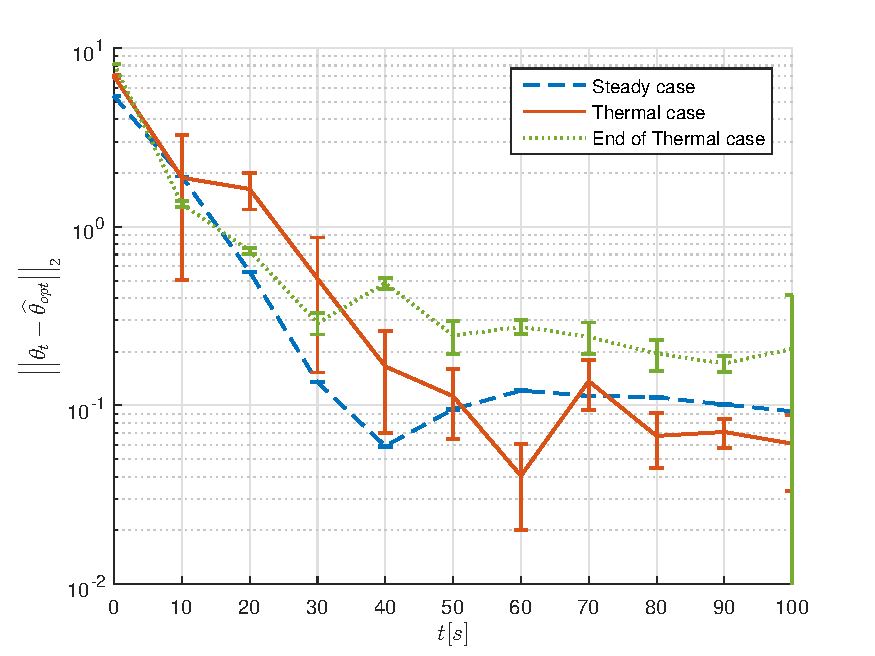
\includegraphics[width=9cm]{img/cv_speed.pdf}
\end{center}
\caption{Convergence of the action-value function}
\label{fig:param_cv}
\end{figure}

The performance reached by the control algorithm can be measured via the total energy of the aircraft, capturing the reached altitude and the velocity. In the three aforementioned scenarios, the expected results are not the same. Indeed, in a steady atmosphere, the optimal policy only allows to minimize the loss of altitude by setting $\beta = \mu = 0$. Such a configuration is optimal since no thermals can be found and the glider can only maximize its long term energy by flying straight and avoiding sharp manoeuvres. Then, when a thermal is reached, the algorithm's exploratory behavior allows to captures the information that it is worth changing $\beta$ and $\mu$, and adapts the trajectory to maximize the long-term return. In the third situation, when the glider flies inside a dying thermal, the algorithm brings back the parameters to a steady atmosphere configuration and again minimizes the expected loss of energy.

%\begin{figure}
%\begin{center}
% 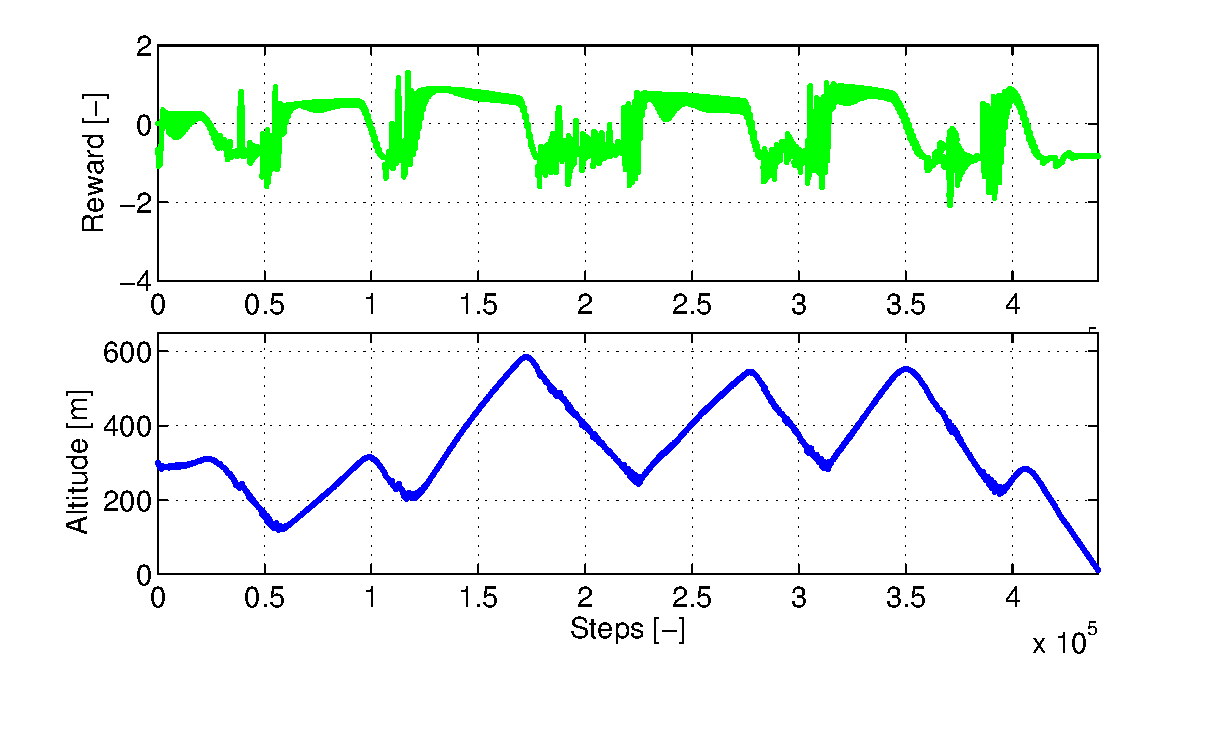
\includegraphics[width=9cm]{img/valid_reward_multi.pdf}
%\end{center}
%\caption{Evolution of reward and altitude}
%\label{fig:evolution_rwd_alti}
%\end{figure}

\begin{figure}
\begin{center}
 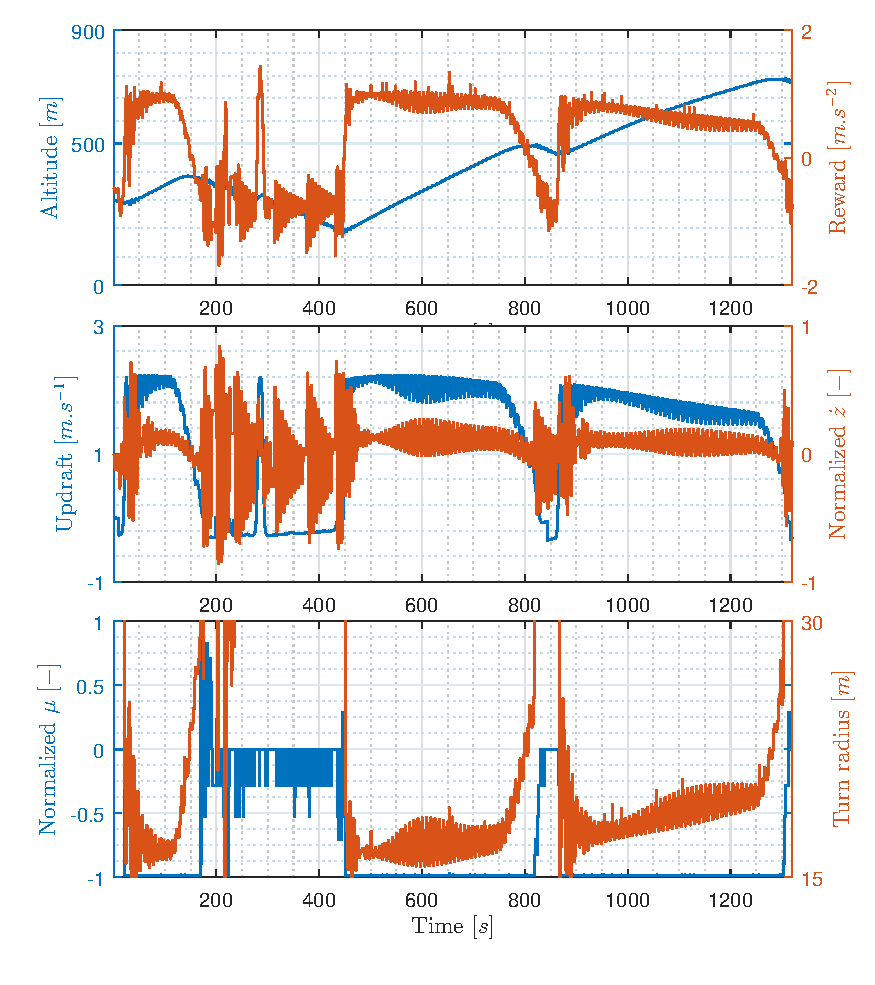
\includegraphics[width=9cm]{img/traj_var.pdf}
\end{center}
\caption{Evolution of the aircraft variables with time}
\label{fig:traj_rho}
\end{figure}

Figure \ref{fig:traj_rho} shows the evolution of altitude and instantaneous rewards through time in a typical long-term scenario with multiple thermal crossings. Each altitude pike shows the entry of the aircraft into a thermal. First the trajectory is bent in order to maximize the altitude gain and when the thermal dies, the glider goes back to the steady flight configuration. Clearly, each gain-of-altitude phase corresponds to a positive reward and, conversely, a loss-of-altitude phase to a negative one. A 3D display of the trajectory inside a thermal is presented in Figure \ref{fig:traj_high_alt}.

\begin{figure}
\begin{center}
 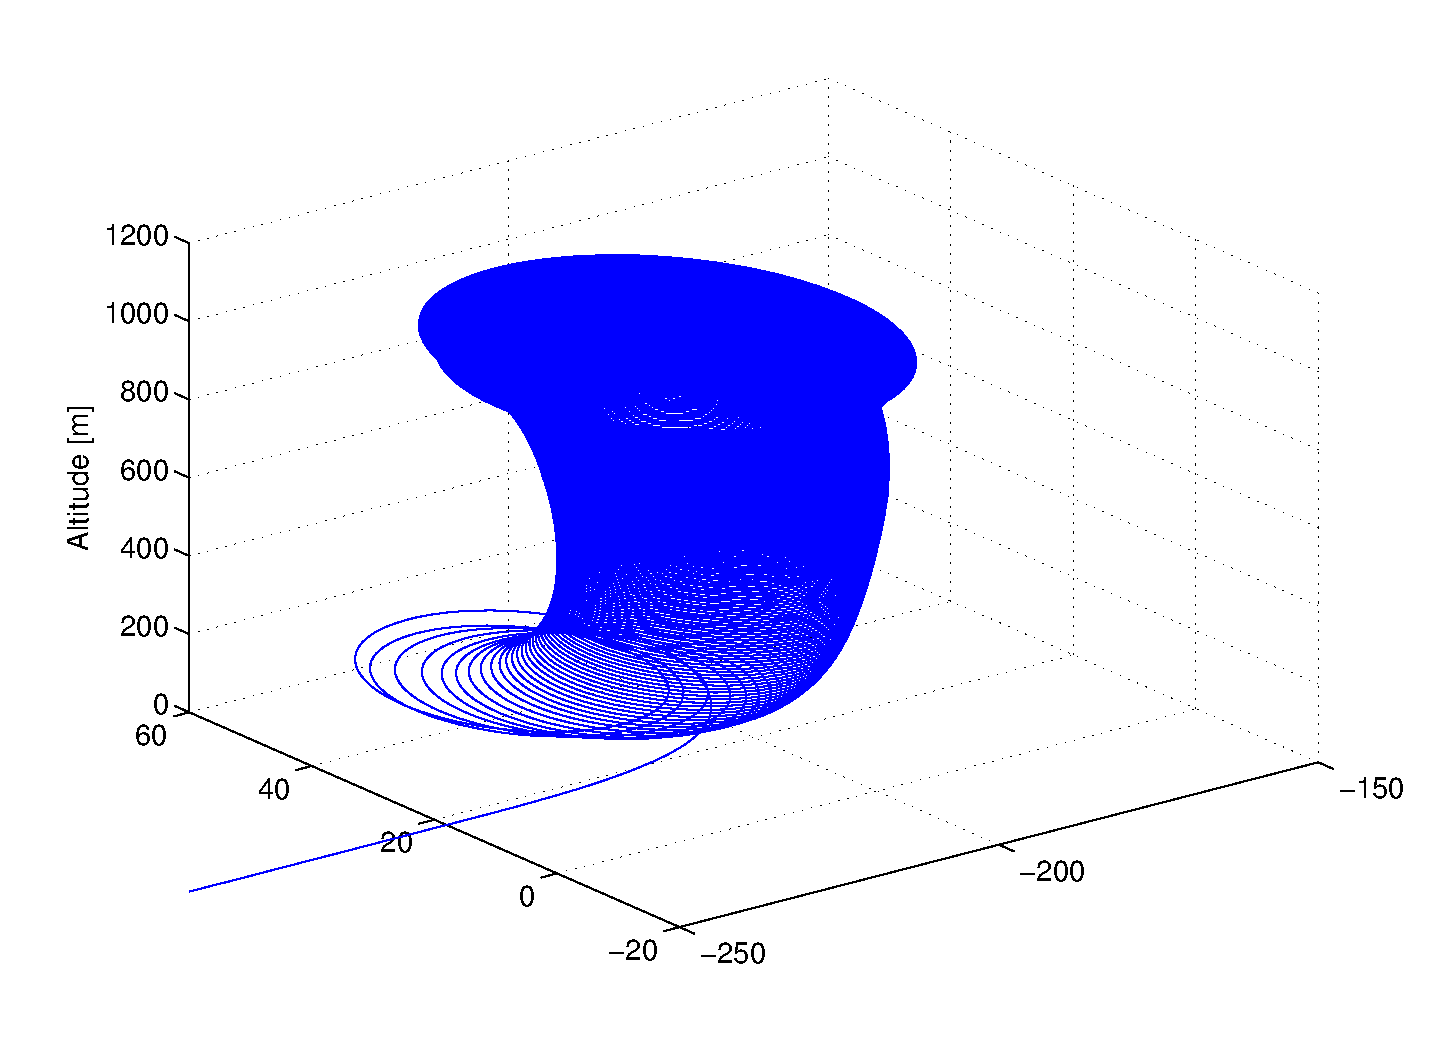
\includegraphics[width=9cm]{img/traj_high_alt.pdf}
\end{center}
 \caption{Trajectory of the aircraft inside a thermal}
 \label{fig:traj_high_alt}
\end{figure}

The $Q$-learning controller yields an overall behaviour close to the one of a human pilot while being totally unaware of its own location and of local wind field models. When flying in still air, the glider remains in ``flat'' flight attitude, thus maximizing its flight time expectancy. Whenever an updraft is spotted, it engages in a spiral, as shown in Figure \ref{fig:traj_rho}. If the updraft dies, the aircraft comes back to the first configuration. This results in an overall trajectory composed with straight lines and circles as displayed in Figure \ref{fig:full_traj}.

\begin{figure}
\begin{center}
 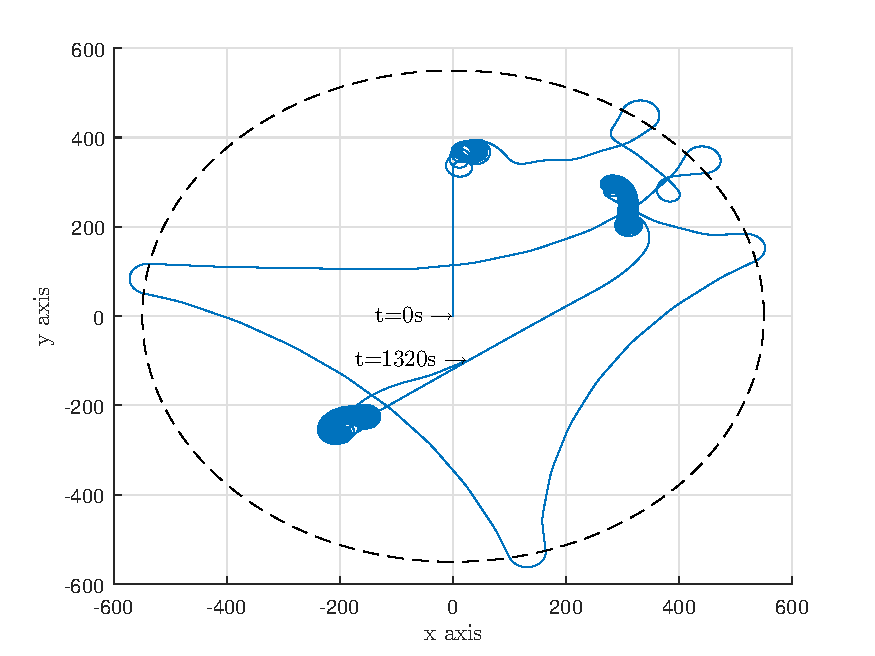
\includegraphics[width=9cm]{img/full_traj.pdf}
\end{center}
\caption{An example of trajectory}
\label{fig:full_traj}
\end{figure}

Figure \ref{fig:traj_rho} also illustrates the reaction times of the glider and the overall command behaviour. It appears that the glider starts to circle up the thermals long before the value function has converged. Similarly, the convergence to a steady air optimal behaviour is faster than the $Q$-function convergence illustrated on Figure \ref{fig:param_cv}.
%It also appears that when the glider reaches the thermal's top, since the updraft decreases at this altitude, it reduces its bank angle (enlarges its turning radius) in order to stay in the thermal while reaching a zero vertical velocity.
When the glider reaches the thermal's top, the updraft naturally decreases. Consequently one can notice the reduction of the bank angle (enlargement of the turning radius) computed by the algorithm in order to stay in the thermal while reaching a zero vertical velocity.

%We measured the autonomy gain obtained by introducing our $Q$-learning controller, against a passive gliding situation, to insure we were not degrading the overall flight autonomy. This measure was obtained by averaging the flight time over ZZZ roll-outs of the system. The average duration of passive flights was $AAA$s against $BBB$s with Q-learning, thus yielding a CCC\% improvement in mission autonomy.

\section{DISCUSSION AND CONCLUSION}
\label{sec:conclu}

In this paragraph, we discuss the limitations of our contribution, highlight directions for improvements and underline how our results make a difference compared to related work in the literature presented in Section \ref{sec:relwork}. To summarize, we implemented a proof of concept that a computationally light algorithm like $Q$-learning could be adapted to take into account the time-varying conditions of thermal soaring flight and could make efficient online changes to the control behavior of an autonomous glider. We take a critical look at this contribution.

First of all, we did not introduce a new RL algorithm \emph{per se}, even though we shortly discuss the question of learning in unsteady environments. The choice of $Q$-learning is justified by its low computational footprint, despite the existence of a vast literature of efficient algorithms in online RL. Our contributions on the RL side are application-specific: first we justify the need for constant $\alpha$ and $\epsilon$ parameters to account for permanent exploration and adaptation in unsteady environments. Secondly, the contribution lies in the relevant choice in state and action variables, such that, under an optimal policy, the system remains in a quasi-constant state (it would not be the case if $x,y,z$ were part of the state space for instance), thus limiting the need for exploration and making the learning process faster. Finally, we introduced a reward model based explicitly on the maximization of the long term energy of the aircraft, thus linking energetic considerations with the definition of the $Q$-function.

From a low-level control point of view, the hypothesis of a control frequency of 1kHz is somehow questionable and it should be decreased in further developments. We argue however that this frequency is representative of a measurement frequency and should thus still be used to update the $Q$-function. Exploratory actions artificially account for the information collected due to the noise in wind conditions felt by the aircraft.

The 6 degrees of freedom aircraft model used in the simulation is a classical flight dynamics model that does not take into account the wind gradient in the wingspan direction. This gradient however is known to be a crucial information for human pilots, since it disambiguates whether a thermal center is on the left or right hand side of the glider. Exploiting such information could bring more efficiency to the glider's control and avoid missing some thermals because the turn was initiated in the wrong direction.

Lastly, in this proof of concept, we based the action space on the aerodynamic angles $\mu$ and $\beta$ as it was done in \cite{dynamic}. Since the $Q$-learning algorithm aims at maximizing the average energy gain in the long term, it does not improve the short-term stabilization of the longitudinal modes of the aircraft, leading to the oscillations shown in Figure \ref{fig:traj_rho}. Even though this does not affect the overall long-term energy gains, a desirable improvement would consist in implementing a low-level stabilization loop (with a PID controller for instance), thus allowing to define the action space using aircraft attitude set points, rather than aerodynamic angles.

Overall, our contribution is three-fold. First we report on how to efficiently adapt a $Q$-learning algorithm to the non-steady, partially observable, control problem of thermal soaring. Then we empirically evaluate the performance of this algorithm in a rich simulation environment, illustrating how it can be used to improve the energy autonomy of soaring planes. Finally we discuss the strengths and limitations of this approach, thus opening research perspectives on this topic and providing first insights on these perspectives.

%% \section{LIMITATIONS}
%% \label{sec:limit}
%% 
%% %TODO
%% 
%% One weakness of our current implementation is the \textit{bouncing} phenomenon, i.e. the fact that sometimes the glider literally bounces on a thermal instead of circling inside. This is due to the random action exploration strategy that initiates the turn in the wrong direction. For instance, if the thermal is on the right and the aircraft turns left without trying to turn right first, it starts gaining energy but quickly flies away and comes back to the steady configuration. This pitfall is well known to glider pilots that adapt their trajectory accordingly while our controller currently just flies away.
%% 
%% It should also be noted that no low-level dampening control of the angle of attack was performed in our simulations. This resulted in the oscillations appearing in Figure \ref{fig:traj_rho}, typical of a phugoid mode. Future work could include such attitude stabilization systems to increase the efficiency of the glider's flight.
%% 
%% \section{CONCLUSION}
%% \label{sec:conclu}
%% 
%% Model-free online reinforcement learning approaches are convenient control methods that present a great adaptivity feature and do not need pre-computation. This proof-of-concept demonstrated their applicability to the problem of maximizing the flight autonomy of a soaring UAV for a low computational cost and no energy consumption. Simulations showed the benefit of an adapted $Q$-learning algorithm in an unknown, unsteady, noisy environment with time and space-dependent updraft velocities. Our intention was to stick to a realistic scenario where updrafts positions are unknown and the policy has to trade-off exploration of the map and exploitation of thermals while maximizing the altitude of the aircraft.
%% 
%% Limits in terms of exploration were met in what we called the \textit{bouncing} phenomenon, suggesting to improve the information collected by the system or their processing, for instance by computing a belief over the environment configuration. This opens the door to a whole span of perspectives, from the left/right disambiguation in the bouncing phenomenon to more advanced function approximation methods in RL, from softer constraints on the control frequencies to different control algorithms and architectures (oscillation damping, simulation-based open-loop online control, actor-critic architectures, policy gradients, etc.). Moreover, future work should explore the interaction between low-level piloting such as the one presented here and the issues in navigation and in mission planning.

\bibliography{mybiblio}

%\begin{thebibliography}{99}
%%\providecommand{\natexlab}[1]{#1}
%%\providecommand{\url}[1]{\texttt{#1}}
%%\providecommand{\urlprefix}{URL }
%%\expandafter\ifx\csname urlstyle\endcsname\relax
%%\providecommand{\doi}[1]{doi:\discretionary{}{}{}#1}\else
%%\providecommand{\doi}{doi:\discretionary{}{}{}\begingroup
%%\urlstyle{rm}\Url}\fi
%
%\bibitem{allen05}
%Allen, M.J. (2005).
%\newblock Autonomous soaring for improved endurance of a small uninhabited air vehicle.
%\newblock Technical report, NASA Dryden Research Center.
%
%\bibitem{allen_thermal}
%Allen, M.J. (2006).
%\newblock Updraft model for development of autonomous soaring uninhabited air vehicles.
%\newblock Technical report, NASA Dryden Flight Research Center.
%
%\bibitem{allen07}
%Allen, M.J. and Lin, V. (2007).
%\newblock Guidance and control of an autonomous soaring uav.
%\newblock Technical report, NASA Dryden Flight Research Center.
%
%\bibitem{dynamic}
%Beeler, S., Moerder, D., and Cox, D. (2003).
%\newblock A flight dynamics model for a small glider in ambient winds.
%\newblock Technical report, NASA.
%
%\bibitem{bencatel13}
%Bencatel, R., de~Sousa, J.T., and Girard, A. (2013).
%\newblock Atmospheric flow field models applicable for aircraft endurance extension.
%\newblock \emph{Prog. in Aerospace Sciences}, 61.
%
%\bibitem{chakrabarty}
%Chakrabarty, A. and Langelaan, J. (2010).
%\newblock Flight path planning for uav atmospheric energy harvesting using heuristic search.
%\newblock In \emph{AIAA Guidance, Navigation, and Control Conference}.
%
%\bibitem{chen1981}
%Chen, M. and McMasters, J. (1981).
%\newblock From paleoaeronautics to altostratus - a technical history of soaring.
%\newblock In \emph{AIAA Aircraft Systems and Technology Conference}.
%
%\bibitem{chen11}
%Chen, W. and Clarke, J.H.A. (2011).
%\newblock Trajectory generation for autonomous soaring {UAS}.
%\newblock In \emph{17th International Conference on Automation and Computing}.
%
%\bibitem{hachiya10}
%Hachiya, H. and Sugiyama, M. (2010).
%\newblock Feature selection for reinforcement learning: Evaluating implicit state-reward dependency via conditional mutual information.
%\newblock In \emph{European Conference on Machine Learning and Knowledge Discovery in Databases}, 474--489.
%
%\bibitem{kahveci}
%Kahveci, N. and Mirmirani, M. (2008).
%\newblock Adaptive {LQ} control with anti-windup augmentation to optimize {UAV} performance in autonomous soaring application.
%\newblock In \emph{IEEE Transactions on Control System Technology}.
%
%\bibitem{lawrance_phd}
%Lawrance, N. (2011).
%\newblock \emph{Autonomous Soaring Flight for Unmanned Aerial Vehicle}.
%\newblock Ph.D. thesis, The University Of Sydney.
%
%\bibitem{lawrance11}
%Lawrance, N. and Sukkarieh, S. (2011).
%\newblock Path planning for autonomous soaring flight in dynamic wind.
%\newblock In \emph{IEEE International Conference on Robotics and Automation}.
%
%\bibitem{nguyen13}
%Nguyen, T., Li, Z., Silander, T., and Leong, T.Y. (2013).
%\newblock Online feature selection for model-based reinforcement learning.
%\newblock In \emph{Int. Conf. on Machine Learning}.
%
%\bibitem{parr08}
%Parr, R., Li, L., Taylor, G., Painter-Wakefield, C., and Littman, M.L. (2008).
%\newblock An analysis of linear models, linear value-function approximation, and feature selection for reinforcement learning.
%\newblock In \emph{International Conference on Machine Learning}.
%
%\bibitem{puterman}
%Puterman, M.L. (2005).
%\newblock \emph{Markov Decision Processes: Discrete Stochastic Dynamic Programming}.
%\newblock John Wiley \& Sons, Inc.
%
%\bibitem{reichmann}
%Reichmann, H. (1993).
%\newblock \emph{Cross-Country Soaring}.
%\newblock Soaring Society of America.
%
%\bibitem{robbins1951}
%Robbins, H. and Monro, S. (1951).
%\newblock A stochastic approximation method.
%\newblock \emph{Ann. Math. Statist.}, 22(3), 400--407.
%
%\bibitem{sutton_book}
%Sutton, R.S. and Barto, A.G. (1998).
%\newblock \emph{Reinforcement Learning: An Introduction}.
%\newblock MIT Press.
%
%\bibitem{watkins92qlearning}
%Watkins, C.J.C. and Dayan, P. (1992).
%\newblock {Q}-learning.
%\newblock \emph{Machine Learning}, 8, 279--292.
%
%\bibitem{wharington_phd}
%Wharington, J. (1998).
%\newblock \emph{Autonomous Control of Soaring Aircraft by Reinforcement	Learning}.
%\newblock Ph.D. thesis, Royal Melbourne Institute of Technology.
%
%\end{thebibliography}

\end{document}
